\section{Comparaciones}

\subsection{Benchmarks}
\paragraph{}
A modo de ampliar la cantidad de resultados anteriormente presentados y con intensión de verificar el comportamiento de las heurísticas implementadas a través de test más rigurosos y un poco más universales, nos vimos en la búsqueda de casos de test conocidos o un poco más estandarizados. En esta búsqueda, se dimos con una página en la web, en la cuál hay varios casos de prueba, no sólo para \mc sino también para coloreo, cubrimiento de vértices, entre otros. La página en cuestión es: \url{http://www.nlsde.buaa.edu.cn/~kexu/benchmarks/graph-benchmarks.htm}. En ella no sólo están los casos de prueba utilizados en esta sección para comparar las heurísticas, sino que también figura una explicación de cómo los mismos fueron creados.

\begin{center}
  \begin{tabular}{|c|c|c|c|c|}
  \hline
  Cant. nodos & \mc & Constructivo & Búsqueda local & Tabú Search\\
  \hline
  450 & 30 & 24(14s) & 25(15s) & 24(114s)\\
  \hline
  595 & 35 & 26(36s) & 27(38s) & 27(317s)\\
  \hline
  760 & 40 & 31(82s) & 33(90s) & 31(755s)\\
  \hline
  945 & 45 & 33(165s) & 37(179s) & 34(27.5min)\\
  \hline
  1150 & 50 & 40(315s) & 40(324s) & 40(54min)\\
  \hline
  1272 & 53 & 37(435s) & 40(455s) & 38(79min)\\
\hline
  \end{tabular}
\end{center}

\subsection{Un caso particular}

\paragraph{}
En la búsqueda de ampliar las comparaciones entre los algoritmos, nos vimos en el trabajo de buscar algún ejemplo de grafo, si es que había, en el cuál se vieran plasmadas las mejoras que se van realizando ejercicio a ejercicio. Por esta razón, se realizó un análisis más detallado del comportamiento de cada algoritmo para ver si se podía cumplir con este objetivo.

\paragraph{}
Luego de realizar varios bosquejos, dimos con el siguiente grafo:

\vspace*{1cm}

\begin{figure}[htb]
  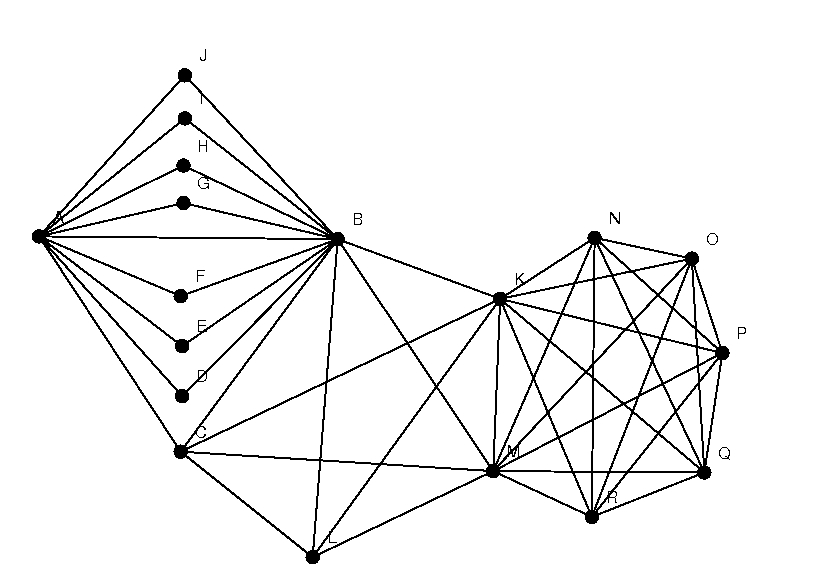
\includegraphics[scale=0.6]{./otros/pruebaDeMejoras.jpg}
  \caption{Grafo en el que se observan distintos resultados entre los distintos algoritmos. Hay una cantidad total de 18 nodos.}
  \label{pruebademejoras}
\end{figure}
\clearpage
\vspace*{2cm}

\paragraph{}
Cabe aclarar que el \mc dentro de este grafo particular es de tamaño 7. Si se hace una corrida de máquina para cada algoritmo implementado en este trabajo práctico sobre este grafo, se observan los siguientes resultados:

\vspace*{2cm}

\begin{table}
  \centering
  \begin{tabular}{|c|c|c|}
  \hline
  \textbf{Algoritmo} & \textbf{\mc encontrada}\\
  \hline
  Exacto & 7\\
  \hline
  Constructivo &3\\
  \hline
  Búsqueda local & 5\\
  \hline
  Búsqueda tabú & 7\\
  \hline
  \end{tabular}
\caption{\mc encontrada por cada algoritmo para el grafo de la Figura \ref{pruebademejoras}.}
\end{table}

\vspace*{1cm}

\paragraph{}
Como se puede ver en esta tabla, existe una mejora en el resultado arrojado por cada heurística. Esto se debe principalmente a las técnicas algorítmicas utilizadas en cada ejercicio, y además a que tanto la heurística de búsqueda local implementada, como la de búsqueda tabú, parten de una solución inicial, que es la arrojada por el algoritmo constructivo. Por lo tanto, partiendo de ese detalle, sabemos que siempre va a valer que:

\begin{equation}
 \#CliqueConstructiva \le \#CliqueBusqLocal \le \#CliqueExacta
\label{mejoras1}
\end{equation}

y

\begin{equation}
 \#CliqueConstructiva \le \#CliqueBusqTabu \le \#CliqueExacta
\label{mejoras2}
\end{equation}

\paragraph{}
Por lo dicho anteriormente, jamás se va a encontrar un ejemplo en el cuál el resultado arrojado por la heurística constructiva sea mayor que el arrojado por cualquiera de las otras heurísticas.\\
El ejemplo de la Figura \ref{pruebademejoras} es un claro ejemplo en el que las desigualdades de las ecuaciones cambian de menor o igual, a estrictamente menor (salvo el caso de la clique exacta y la tabú).

